\documentclass[10pt,a4paper]{article}
\usepackage[utf8]{inputenc}
\usepackage[english]{babel}
\usepackage[T1]{fontenc}
\usepackage{amsmath}
\usepackage{amsfonts}
\usepackage{amssymb}
\usepackage{makeidx}
\usepackage{graphicx}
\usepackage{fourier}
\usepackage{tabularx}
\usepackage[left=2cm,right=2cm,top=2cm,bottom=2cm]{geometry}
\author{Johannes Scheller, Vincent Noculak, Lukas Powalla}
\title{Computational Physics - Project 2}
\begin{document}
\maketitle
\newpage
\tableofcontents
\newpage
\section{Introduction And Motivation}
In many fields of both mathematics and physics, we often come to the point that we have to solve so-called eigenvalue problems, which are equations of the form $\hat{A}\cdot\hat{v}=\lambda\hat{v}$, where $\hat{A}$ is a matrix of dimension $n\times n$ and $v$ is a vector of dimension $n$. Equations of this kind occur not only in linear algebra, but also in mechanics and quantum mechanics and will also be a major part of this report. In this project, we are going to rewrite the Schrödinger's equation of one and two electrons in a harmonic oscillator potential in the form of an eigenvalue problem and solve it numerically by implementing Jacobi's method, an algorithm that can be used to solve any eigenvalue problem.

\section{Theory}
\subsection{Rewriting Schrödinger's equation as eigenvalue problem}
\subsubsection{One electron in a harmonic oscillator potential}
\subsubsection{Two interacting electrons in a harmonic oscillator potential}
\subsection{Jacobi's method}
\section{Execution}
\subsection{Implementing the algorithm}
\subsection{Setting and Testing of Parameters}
%Check this section again!
In both cases, whether we deal with only one particle or with two, we have three parameters to be set, resulting in two degrees of freedom that have an effect on the accuracy of our results. The first and most obvious parameter is $n$, the number of grid points we use. Using a higher value of $n$, we gain more precision as the step length decreases, but at the same time, we will end up with a larger matrix that needs more memory (proportional to $n^2$). Most important, the number of similarity transformations needed to calculate the eigenvalues goes like $n^3$, leading to a very long computation time for large matrices. The highest possible value we used for $n$ was $1000$, resulting in more than 45 minutes of computation time!

The second parameter that we can alter is $\rho_{max}$, the maximum value of $\rho$. In theory, this value should be infinite, which is just not possible for this numeric solution. In our case, the higher an eigenvalue is, the more its calculation depends on the choice of $\rho_{max}$. Therefore the challenge was to set this parameter to a value which resulted in stable and consistent results for the first three eigenvalues without being to high, as a higher value would also increase our step length $h$ if we don't change $n$ accordingly.

The last degree of freedom is to set the tolerance for the non-diagonal matrix elements that are supposed to become zero. This value determines implicitly how many similarity transformations are being operated until the non-diagonal elements are considered zero. A smaller value can lead to higher precision in the eigenvalues, but will at the same time increase the computation time again.

We tested different set-ups with different values of $n$, $rho_{max}$ and $epsilon$ with the results shown in table \ref{parameters}. As we wanted a precision of three leading digits for the three lowest eigenvalues, we decided to use the set-up with $n=$, $rho_{max}=$ and $epsilon=$, which seemed to be a good compromise between precision and computation time and led to the desired results.
%Table here!
\subsection{Results}

By calculating the first three eigenvalues with our Jacobi algorithm for $n = 400$, $\rho_{max} = 6$ and $\epsilon = 10^{-8}$,the values we obtain are 2.99993, 6.99965 and 10.9991. Those eigenvalues match good with the analytical eigenvalue which are 3, 7 and 11.

\begin{figure}[h]
	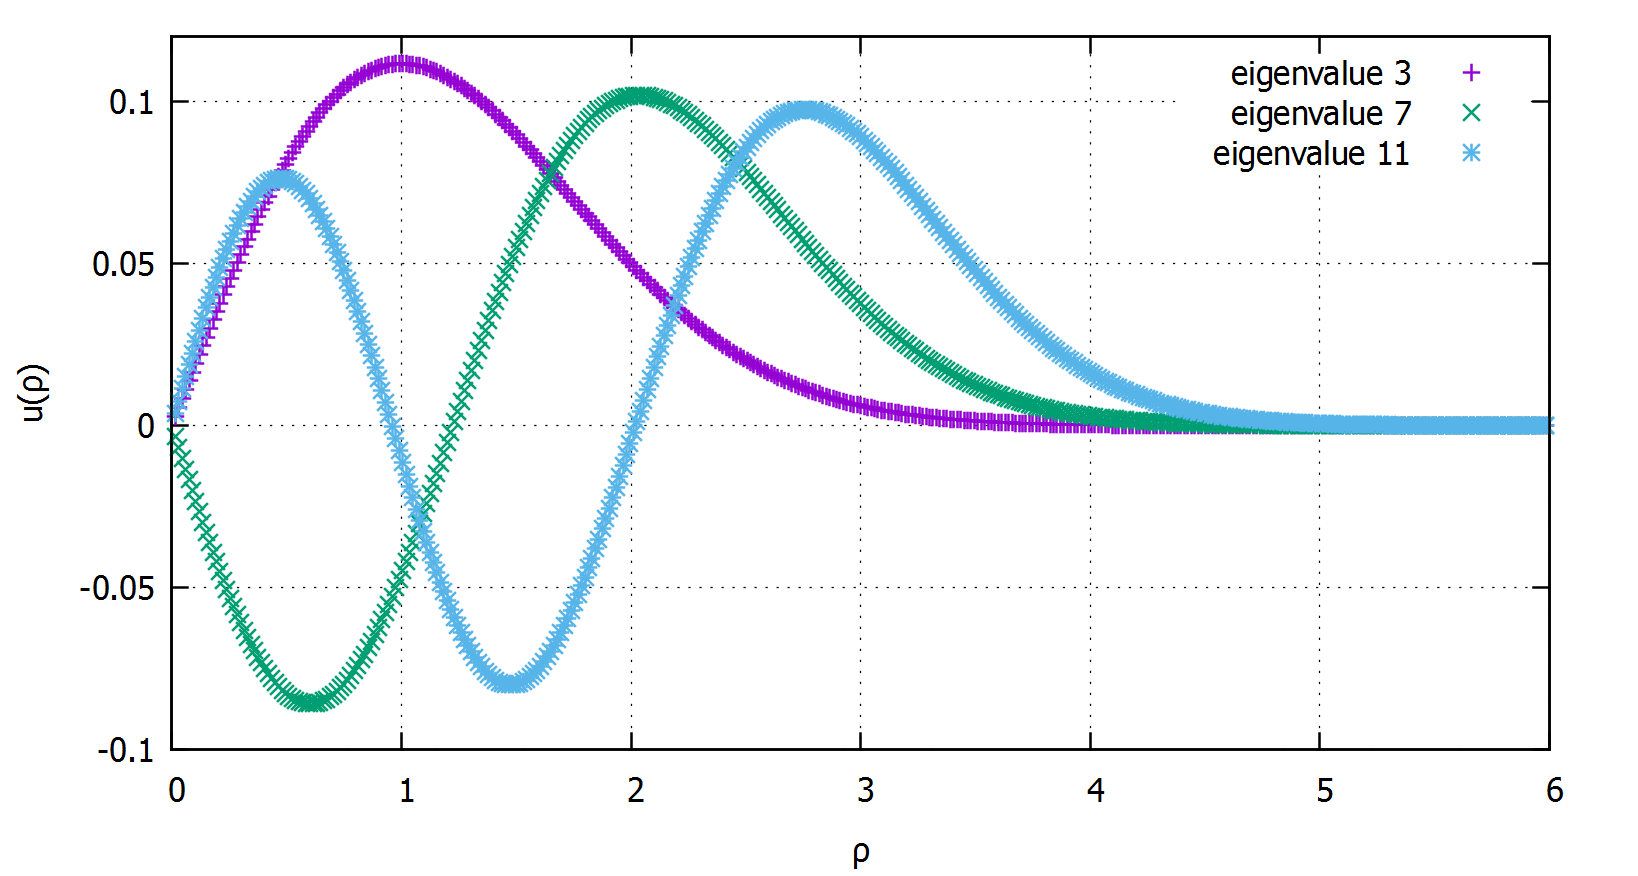
\includegraphics[scale = 0.25]{tvJacobi_comparison_thick.png}
	\centering
	\caption{Functions to different eigenvalues}
	\label{plot1el}
\end{figure}

In figure \ref{plot1el} the functions to these eigenvalues can be seen.

Because the Jacobi algorithm is not specifically designed for triangular matrices like we have, calculating the eigenvalues for a high n requires a lot of iterations. Hence, for higher n, we need a lot of time to calculate the values. In our case it makes more sense to use an algorithm which is designed for a triangular matrix, like Householder`s algorithm. Table \ref{executiontime} backs this up. While the Householder algorithm takes less than two seconds execution time for a matrix with $n = 500$, the time for the Jacobi algorithm increases quickly for bigger n and is already at 696 seconds for $n = 500$.

\begin{table}[h!]
	\centering
	\begin{tabular}{|l|r|c|lrp{16cm}}\hline
		n & Jacobi & Householder\\\hline
		200 & 15s & <1s\\
		250 & 38s & <1s\\
		500 & 696s & 1s\\
		700 & & 5s \\
		1000 & & 24s\\\hline
	\end{tabular}
	\caption{Execution time needed for the Jacobi and Householder algorithm with a nxn matrix }
	\label{executiontime}
\end{table}

Figure \ref{plotiterations} shows the needed iterations for a nxn matrix in our Jacobi algorithm for two different $\rho_{max}$`s. It can be seen that the number of iterations needed is proportional to $n^{2}$. This reflects why the execution time increases that quickly for higher n. While the number of the needed iterations can be approximated with $f(n) = 1.6 \cdot n^2$ for  $\rho_{max} = 10$, we can approximate it just with $g(n) = 0.08 \cdot n^2$ for  $\rho_{max} = 100$. This big decrease in iterations for bigger $\rho_{max}$ is due to the fact that the step length is defined by $h = \frac{\rho_{max}}{n}$. Hence the first non-diagonal matrix elements are given by $e = \frac{n^2}{\rho_{max}^2}$. Because of that the first non-diagonals get rapidly smaller for bigger $\rho_{max}$ and as a consequence all non-diagonal matrix elements are smaller than $\epsilon$ in less similarity transformations. 

\begin{figure}[h]
	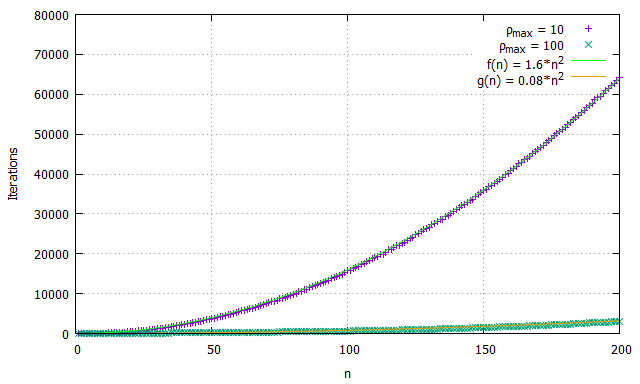
\includegraphics[scale = 0.45]{iterations_comparison_notitle.png}
	\centering
	\caption{Number of iterations needed for a nxn matrix($\epsilon = 10^{-8}$)}
	\label{plotiterations}
\end{figure}

By computing the eigenvalues for two electrons in a harmonic oscillator for different $\omega_{r}$ with $n = 250$ and $\rho_{max} = 3$ we get the results seen in table \ref{ev2el}. When looking at the calculated first eigenvalue for different $\rho_{max}$ and n it can be seen that the value is dependent on those variables. While the first eigenvalue quickly changes for lower n, it stays nearly stable for bigger n which give the better approximation for it. If we choose a $\rho_{max}$ bigger than three, the eigenvalue stays nearly the same, but slowly decreases with increasing $\rho_{max}$. It has to be mentioned that the plot shows very big range of values for $\rho_{max}$. For at least $\rho_{max} = 4$ the function to the first eigenvalue can clearly be seen as 0 as you can see in figure \ref{plot2el2}. Hence the approximation of our algorithm, that we assume $\psi(\rho_{max}) = 0$, is probably not the reason the eigenvalue changes. It is more likely that the direct influence of $\rho_{max}$ on the first non-diagonal element e of the matrix A is the reason for the change of the eigenvalue(like we explained, when we looked at the number of iterations for $\rho_{max} = 100$)

\begin{figure}[h]
	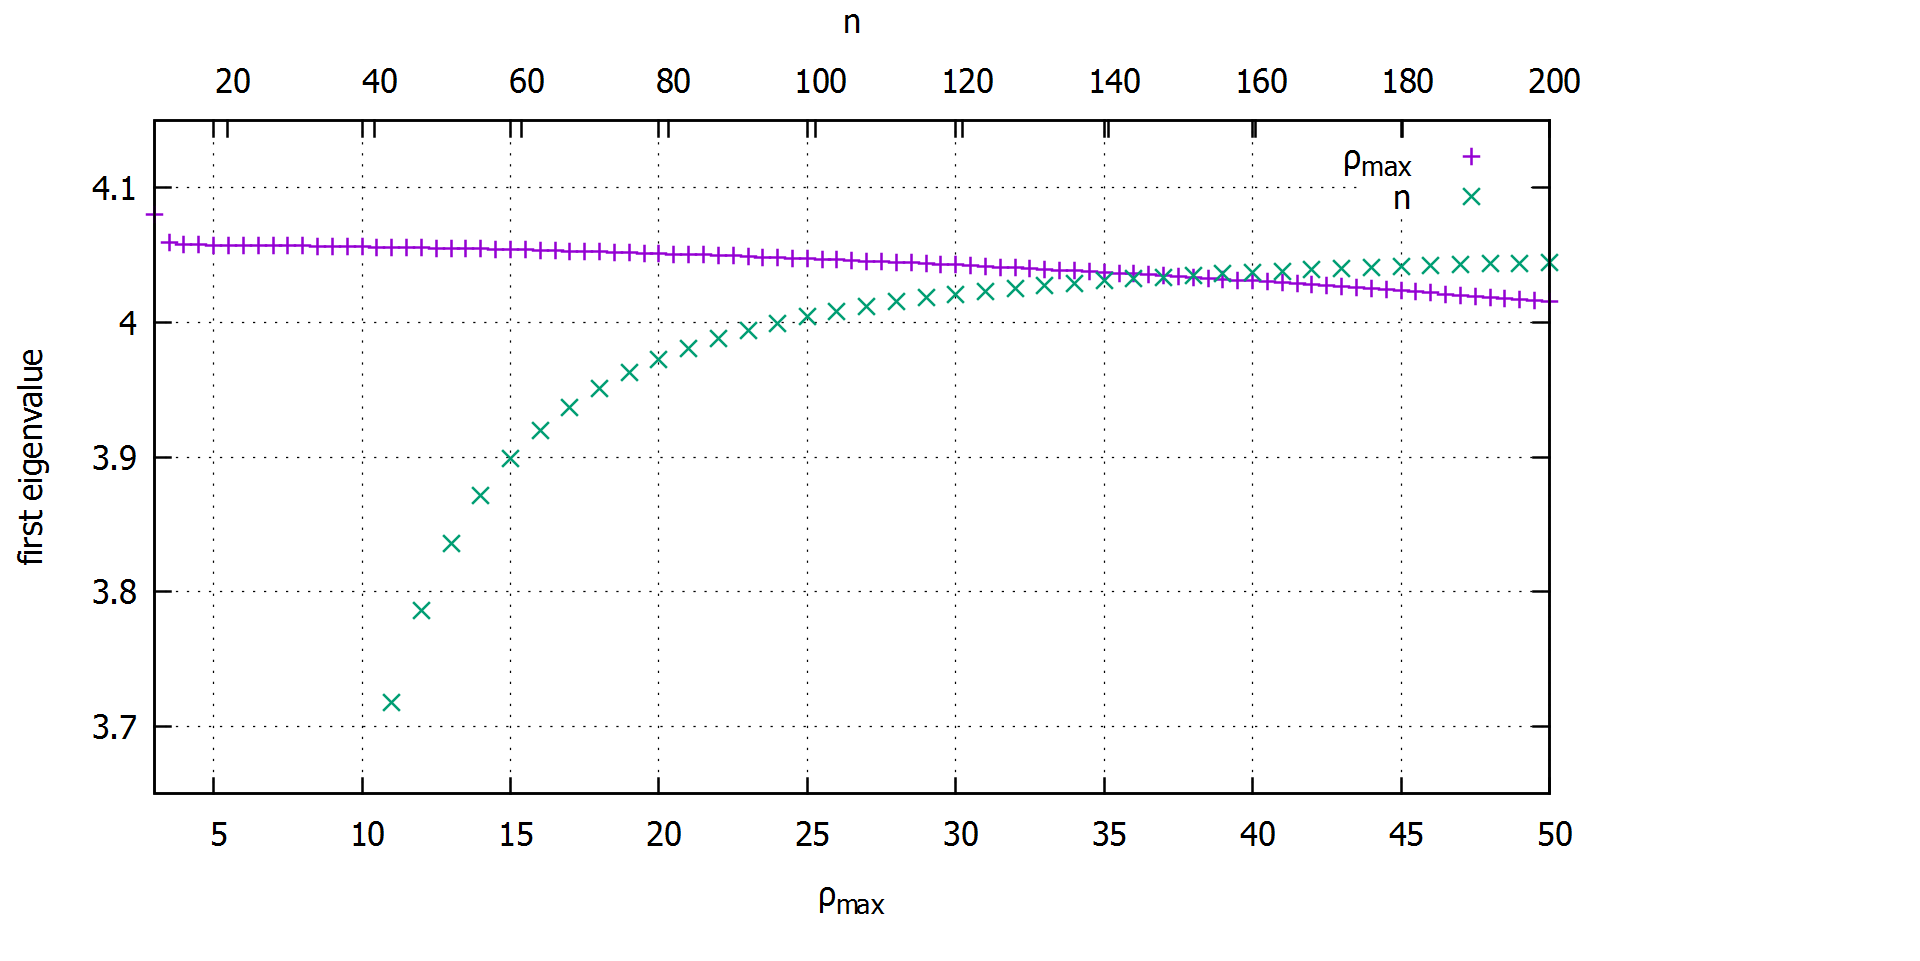
\includegraphics[scale = 0.18]{rhomax_and_n_against_ev.png}
	\centering
	\caption{Dependence of the first eigenvalue of $\rho_{max}$ and n }
	\label{eigenvaluedependence}
\end{figure}

\begin{table}[h!]
	\centering
\begin{tabular}{|l|r|c|lrp{16cm}}\hline
	$\omega_{r}$ & Eigenvalue\\\hline
	0.01 & 0.10577\\
	0.5 & 2.2300\\
	1.0 & 4.0578\\
	5.0 & 17.448\\\hline
\end{tabular}
	\caption{Eigenvalues for different 	$\omega_{r}$}
	\label{ev2el}
\end{table}

\begin{figure}[h]
	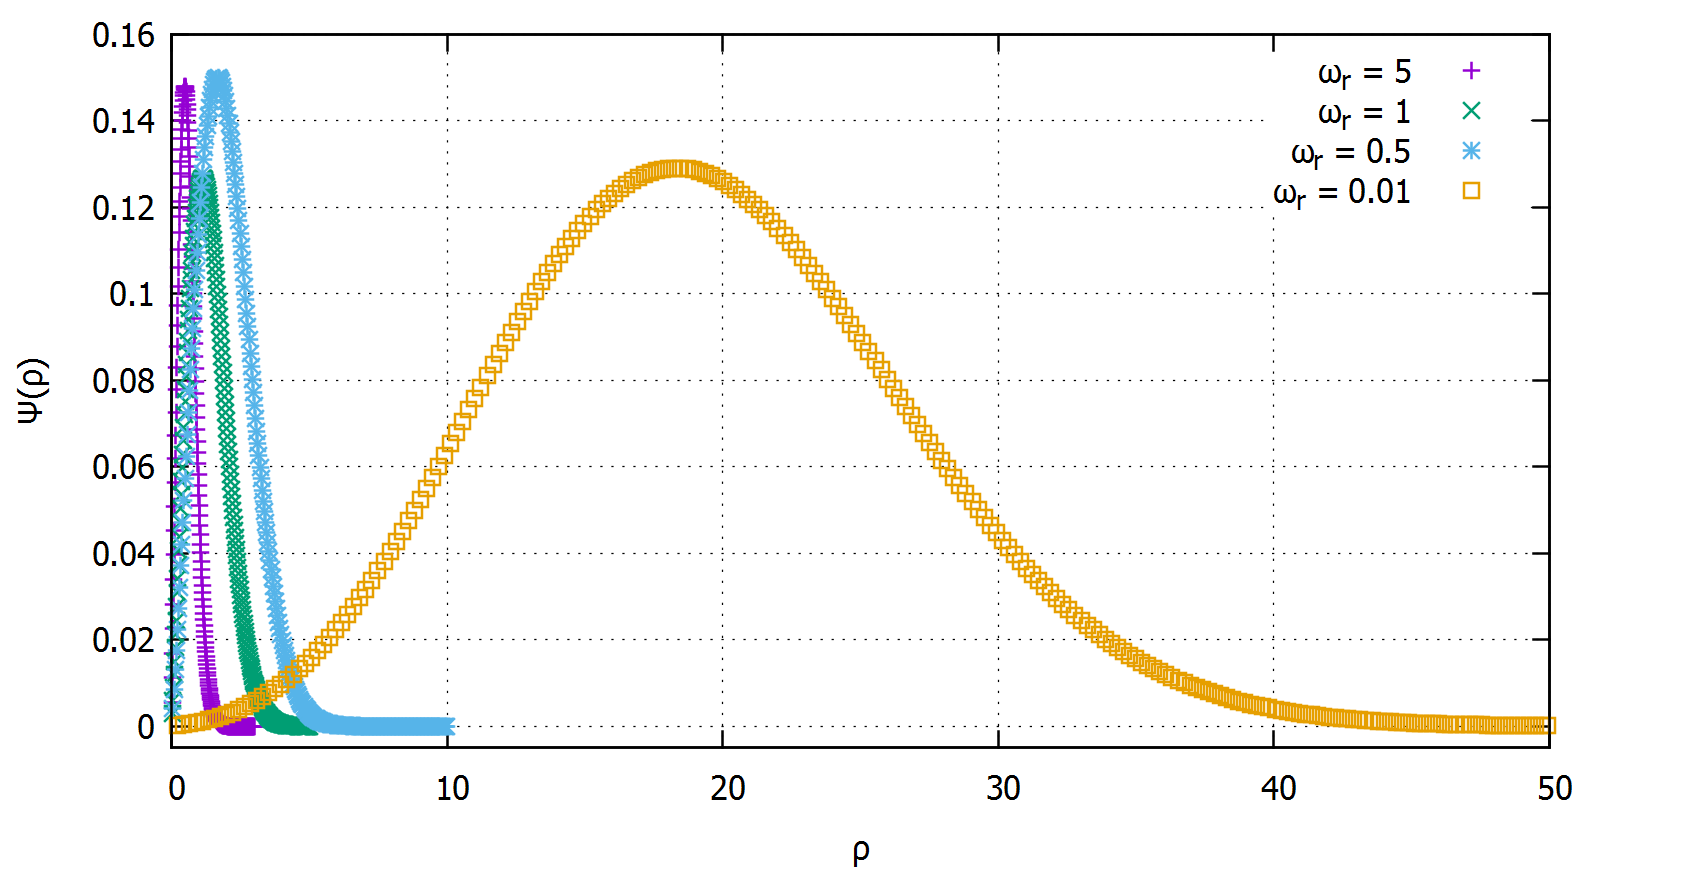
\includegraphics[scale = 0.25]{2Electrons_comparison_thick.png}
	\centering
	\caption{Two electrons in a harmonic oscillator for different $\omega_{r}$`s(1) }
	\label{plot2el1}
	\end{figure}
	
\begin{figure}[h]
	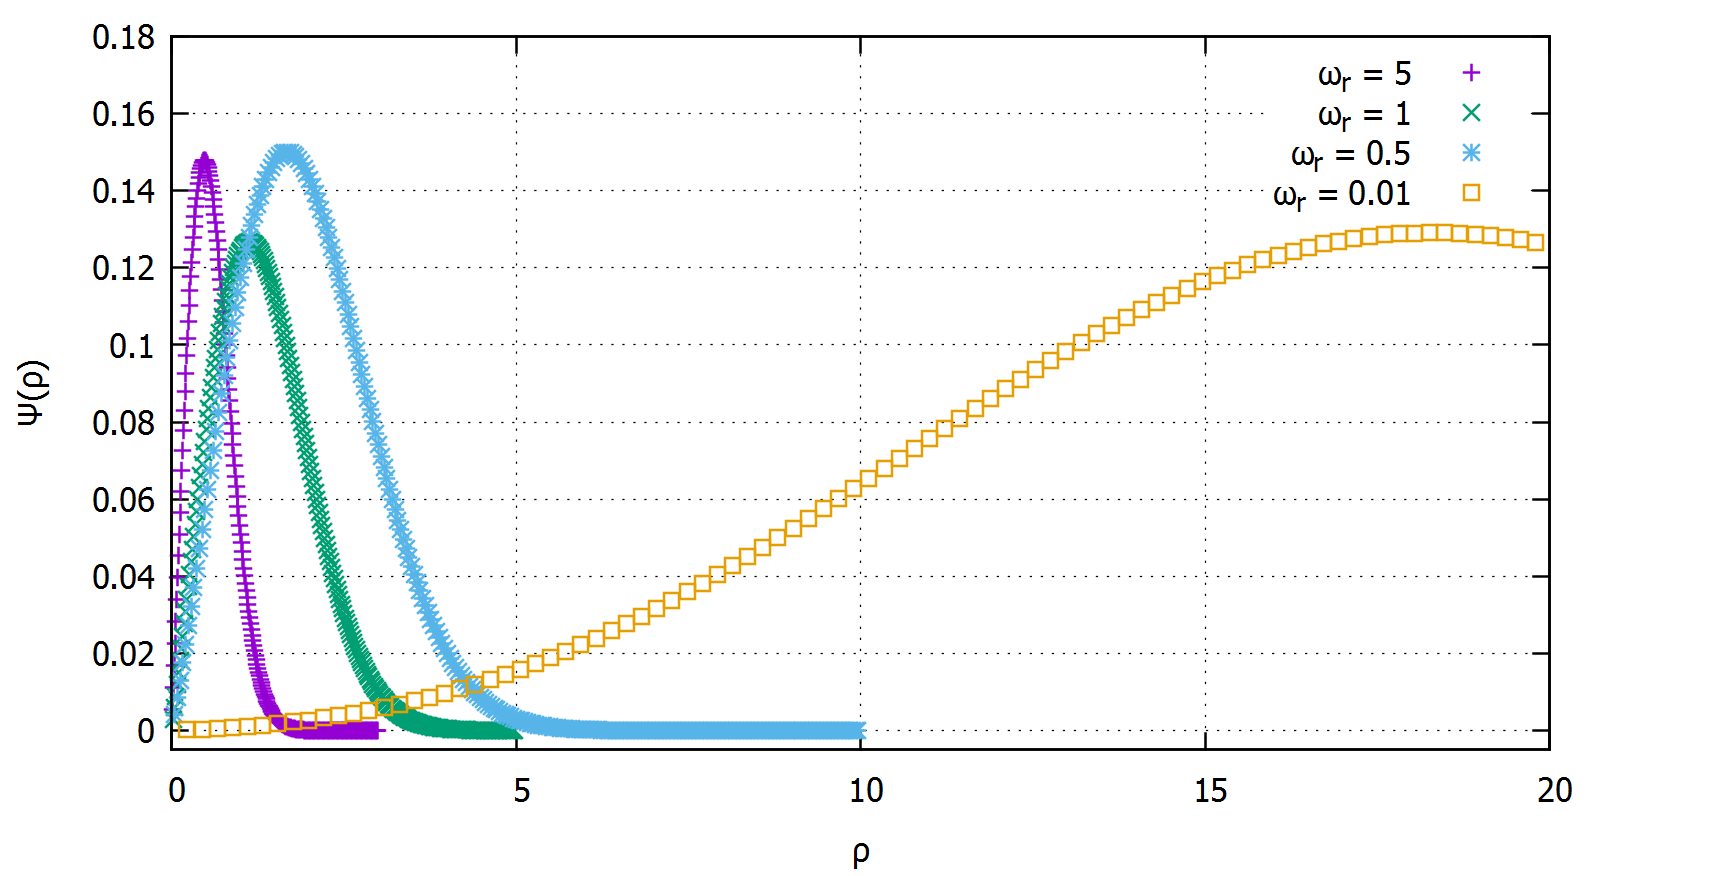
\includegraphics[scale = 0.25]{2Electrons_comparison2_thick.png}
	\centering
	\caption{Two electrons in a harmonic oscillator for different $\omega_{r}$`s(2) }
	\label{plot2el2}
\end{figure}


In figure \ref{plot2el1} and \ref{plot2el2} the functions to the first eigenvalue for different $\omega_{r}$ can be seen. It can be observed that, the smaller $\omega_{r}$ is, the more the eigenfunction gets forced against zero. Hence the average distance between the two electrons gets smaller. One way to interpret this is, that through the increasing potential(which directly depends on $\omega_{r}$) it gets harder for the Coulomb interaction between the electrons to push them apart.

Next we plotted the wave function depending on r in figure \ref{plot2elr}. In this plot it can be seen again, that for a increasing potential(this time we varied it with the variable k) the electrons are more likely to be less distant to each other. It can also be observed that the peak of the wave function gets wider for smaller k.

\begin{figure}[h]
	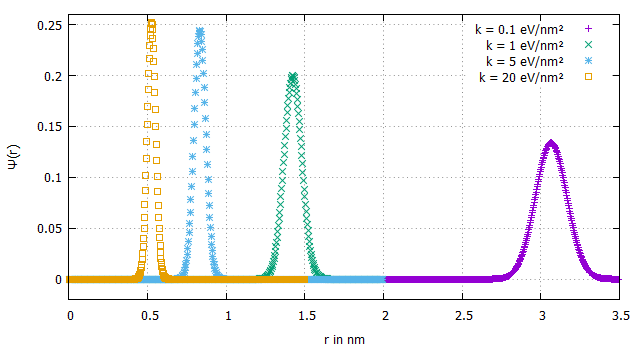
\includegraphics[scale = 0.65]{comparison_different_k_thick.png}
	\centering
	\caption{Two electrons in a harmonic oscillator for different k`s}
	\label{plot2elr}
\end{figure}

\begin{figure}[h]
	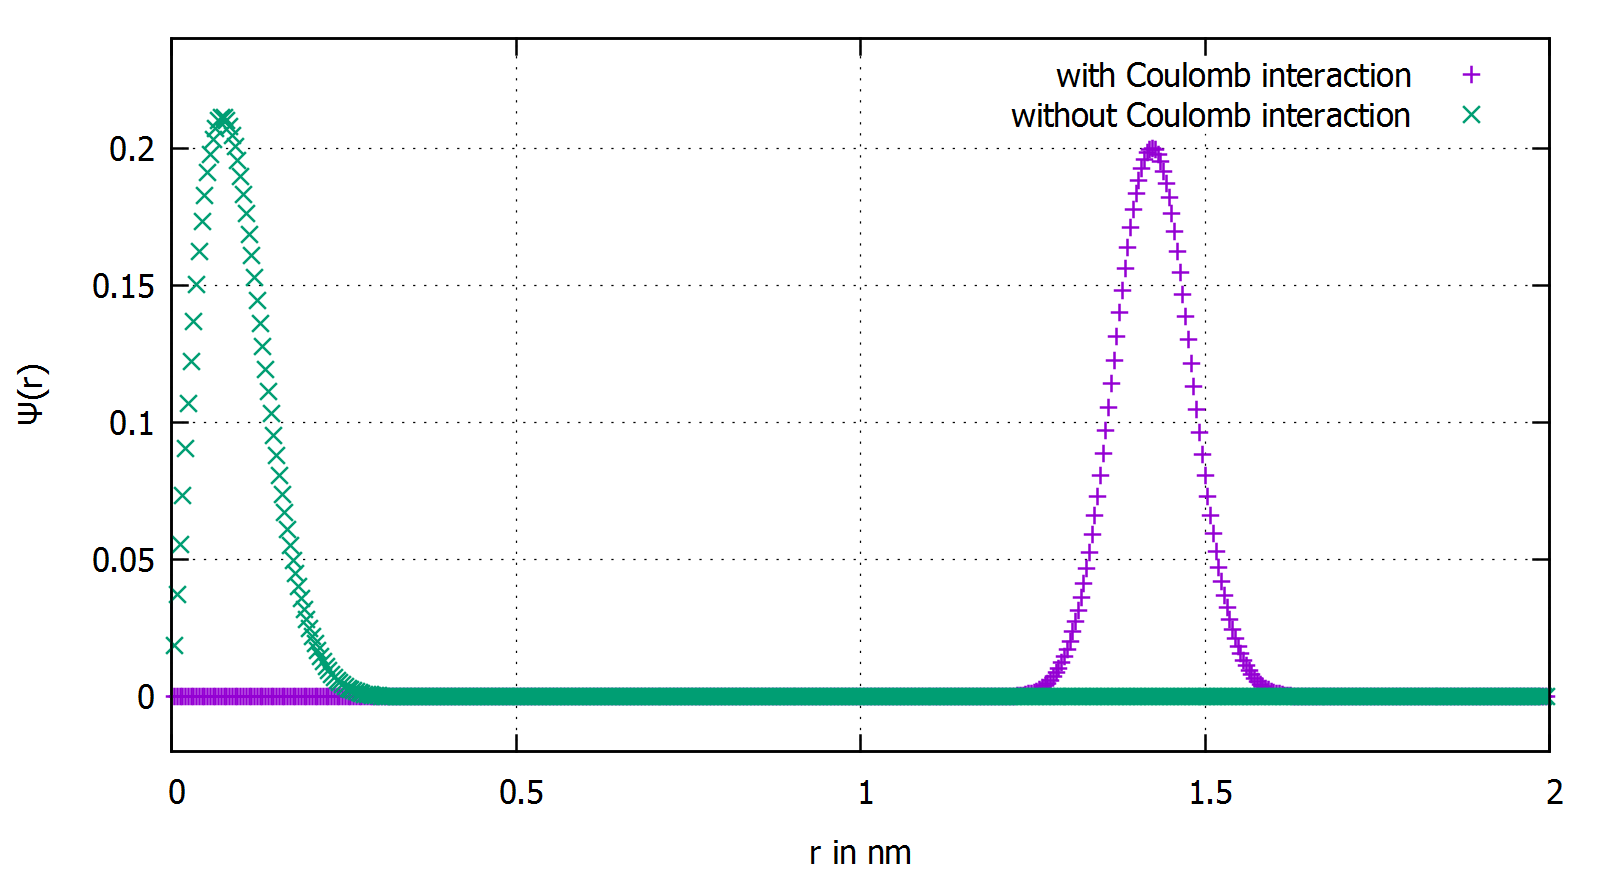
\includegraphics[scale = 0.25]{k1_comparison_2El_n500.png}
	\centering
	\caption{Two electrons in a harmonic oscillator with and without Coulomb interaction}
	\label{plot2elrcoulomb}
\end{figure}

When we now turn off the coulomb interaction between the two electrons(table \ref{plot2elrcoulomb}), we observe that we obtain the same function like when we observed just one electron. Our calculated energies for the first three eigenstates($n = 1100$, $\rho_{max} = 5 nm$) are 1.5206 eV, 1.5254 eV and 1.5301 eV.









\section{Comparison and discussion of the results}
\end{document}